\documentclass[journal=jacsat,manuscript=article]{achemso}
\usepackage[utf8]{inputenc}
\usepackage{graphicx}
\usepackage{subfigure}
\usepackage{amssymb,amsfonts,amsmath}
\usepackage{url}
\usepackage{booktabs, multicol, multirow}

\author{Kyle A. Beauchamp}
\affiliation[Biophysics Program]{Biophysics Program}

\author{Rhiju Das$^\dagger$}
\affiliation[Biochemistry Department]{Biochemistry Department, Stanford University, Stanford, CA}

\author{Vijay S. Pande$^\dagger$}
\affiliation[Chemistry Department]{Chemistry Department, Stanford University, Stanford, CA}

\email{rhiju@stanford.edu, pande@stanford.edu}

\title{Inferring Structural Ensembles from Noisy Experiments: Application to Trialanine}

\begin{document}

\maketitle

\begin{abstract}

Inferring biomolecular conformation from experiment is the fundamental task of structural biology.  Due to limited experimental resolution, structure determination often requires a combination of modeling and experiment.  The vast majority of algorithms for structure determination, however, are limited to modeling a single conformation and provide only limited uncertainty information.  Here we describe Bayesian Energy Landscape Tilting (BELT), a scheme that combines simulation and experiment to infer solution ensembles.  BELT leverages the machinery of Bayesian statistics to give rigorous uncertainty estimates for structural features and equilibrium properties, given simple, well-defined assumptions.  Using trialanine as a test system, we show that BELT corrects force field bias, as measured by $\chi^2$ agreement with trialanine measurements \emph{not used} to fit the models.  BELT modeling with just six NMR measurements estimates $\alpha$, $\beta$, and $PP_{II}$ conformational populations that are 
independent of force field.  

\end{abstract}

\section{Introduction}

Over the past forty years, structural biologists have solved ``ground-state'' structures of countless biological macromolecules\cite{Berman2000}. Modern biology, however, presents many systems that do not fit the single-structure paradigm.  Excited states of nucleic acids\cite{dethoff2012}, natively disordered proteins\cite{fink2005}, and protein folding intermediates\cite{korzhnev2004} alike are poorly described by single conformation models.  For such systems, models of conformational ensembles are required to understand and predict structural and equilibrium properties.  

A growing body of research has sought to understand conformational ensembles.  Much of it has focused on incorporating dynamical information during NMR structure determination \cite{lindorff2005simultaneous, lange2008recognition} or the extraction of multiple conformers from X-ray diffraction data \cite{depristo2004heterogeneity, lang2010automated}.  While these techniques are powerful, they share difficulties in data collection and the unified treatment of heterogeneous experimental data.  At the same time, molecular dynamics studies have demonstrated heterogeneity in the atomic-scale structure of macromolecules \cite{shaw2010}.   However, simulation studies suffer from possible inaccuracies in molecular dynamics force fields, as revealed by benchmarks and optimizations of molecular dynamics force fields \cite{li2011iterative, best2012optimization, lindorff2012systematic}.  In the present work, we connect these two extremes by combining equilibrium experimental measurements with molecular simulation.  

Here we introduce a statistical approach to modeling solution ensembles of biological macromolecules.  The algorithm, Bayesian Energy Landscape Tilting (BELT), uses solution experiments to reweight a collection of atomistic models.  BELT extends a recent maximum entropy method for restraining simulations \cite{chodera2012} to \emph{reweight} existing simulations.  Furthermore, BELT leverages Markov Chain Monte Carlo to transform experimental ambiguity into error bars on arbitrary structural features.  

To validate BELT, we investigate the conformational propensities of trialanine using NMR measurements \cite{Graf2007} and MD simulations performed in five different force fields.  Although the raw simulations show wide variations in their conformational preferences, BELT corrects force field errors to provide self-consistent estimates of the $\alpha$, $\beta$, and $PP_{II}$ populations.  The ability to correct the biases of all tested forcefields suggests that BELT is a powerful technique for connecting simulation and equilibrium measurements.  

\section{Theory: Bayesian Energy Landscape Tilting}

\subsection{Model Inputs}

To model an ensemble using BELT requires three components (Fig. \ref{figure:BELT}).  First, we need conformations $(x_j)_{j=1}^{m}$ sampled from the approximate equilibrium distribution of our system.  In the present work, such conformations will be generated from molecular dynamics simulations.  Second, we require equilibrium experimental measurements $(F_i)_{i=1}^n$ and their associated uncertainties $(\sigma_i)_{i=1}^{n}$.  Third, it is necessary to have a direct connection between simulation and experiment.  This connection is achieved by predicting each experimental observable at each conformation: $f_i(x_j)$ is the predicted value of experiment $i$ at conformation $x_j$.  

\begin{figure}

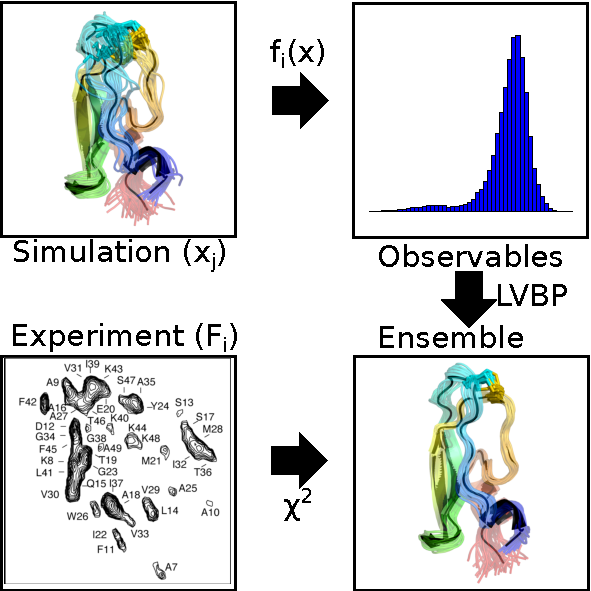
\includegraphics[width=18.0cm]{figures/info_graphic/info_graphic.pdf}

\caption{
General scheme for BELT modeling.
}
\label{figure:BELT}
\end{figure}

\subsection{Reweighting}

The next step in constructing an ensemble is to calculate the population of each conformation.  For convenience, we work with the $\log$ populations (i.e. free energies). Inspired by a previous method for restraining simulations \cite{chodera2012} (see Appx. S1), we reweight individual conformations by a biasing potential that is a linear combination of the predicted observables:

$$\Delta U(x;\alpha) = \sum_i^n \alpha_i f_i(x)$$

In $\Delta U(x;\alpha)$, the parameters $\alpha_i$ determine how strongly each experiment contributes to the biasing potential.  One way to think about $\alpha$ is via ``tilting'' the energy landscape along the order parameters $f_i(x)$.  Given the biasing potential, the population of each conformation can be calculated using exponential averaging (see Appx. S2):

$$\pi_j(\alpha) = \frac{1}{\sum_k \exp[-\Delta U(x_k;\alpha)]} \exp[-\Delta U(x_j;\alpha)]$$

It is informative to consider the case of a single observable $f(x)$.  Suppose the molecule of interest shows a bimodal observable.  If we let $\alpha$ = 0, then the biasing potential is $0$ everywhere and our reweighted ensemble simply returns the results of the MD simulation (Fig. \ref{figure:Hist}b).  If we let $\alpha = -1$, conformations with large values of $f(x)$ are upweighted, while conformations with lower values of $f(x)$ are downweighted (Fig. \ref{figure:Hist}a).  Finally, if $\alpha = 1$, the ensemble shifts in the opposite direction (Fig. \ref{figure:Hist}c).  

\begin{figure}

\subfigure[]{
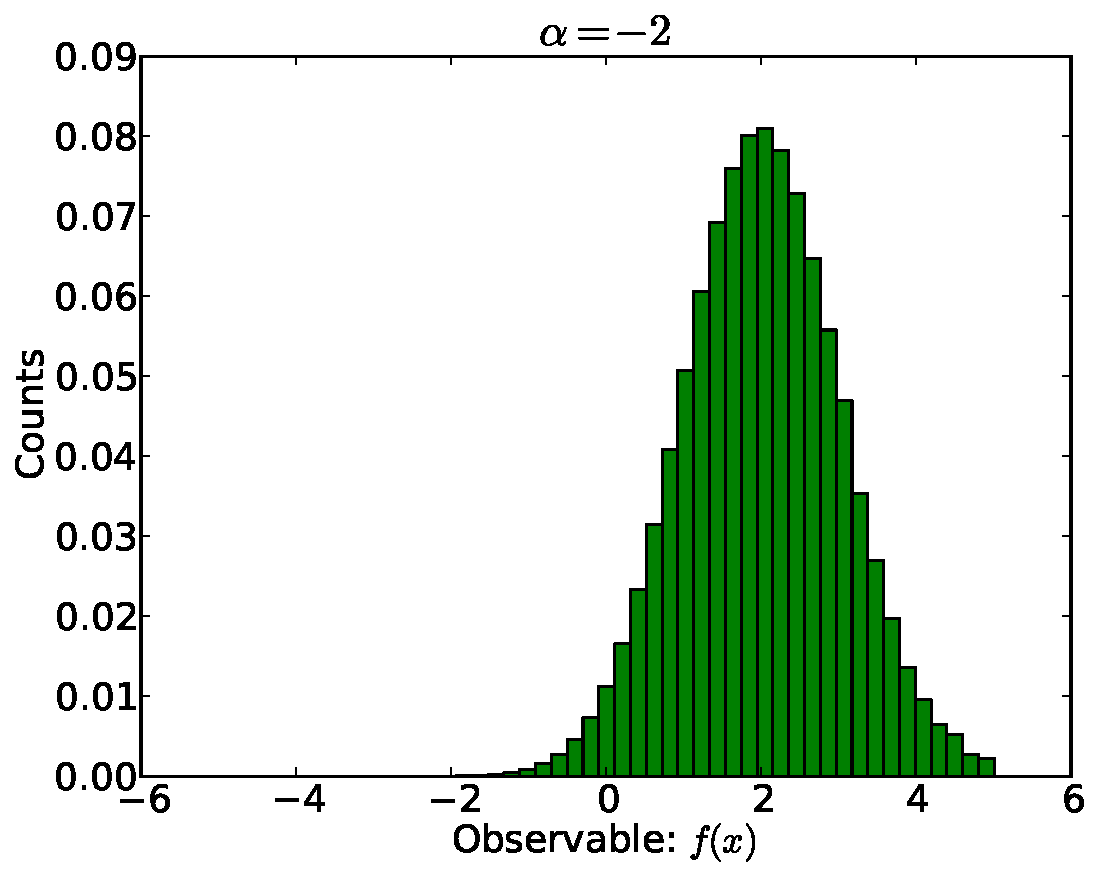
\includegraphics[width=5.0cm]{figures/model_hist-2.pdf}
}
\subfigure[]{
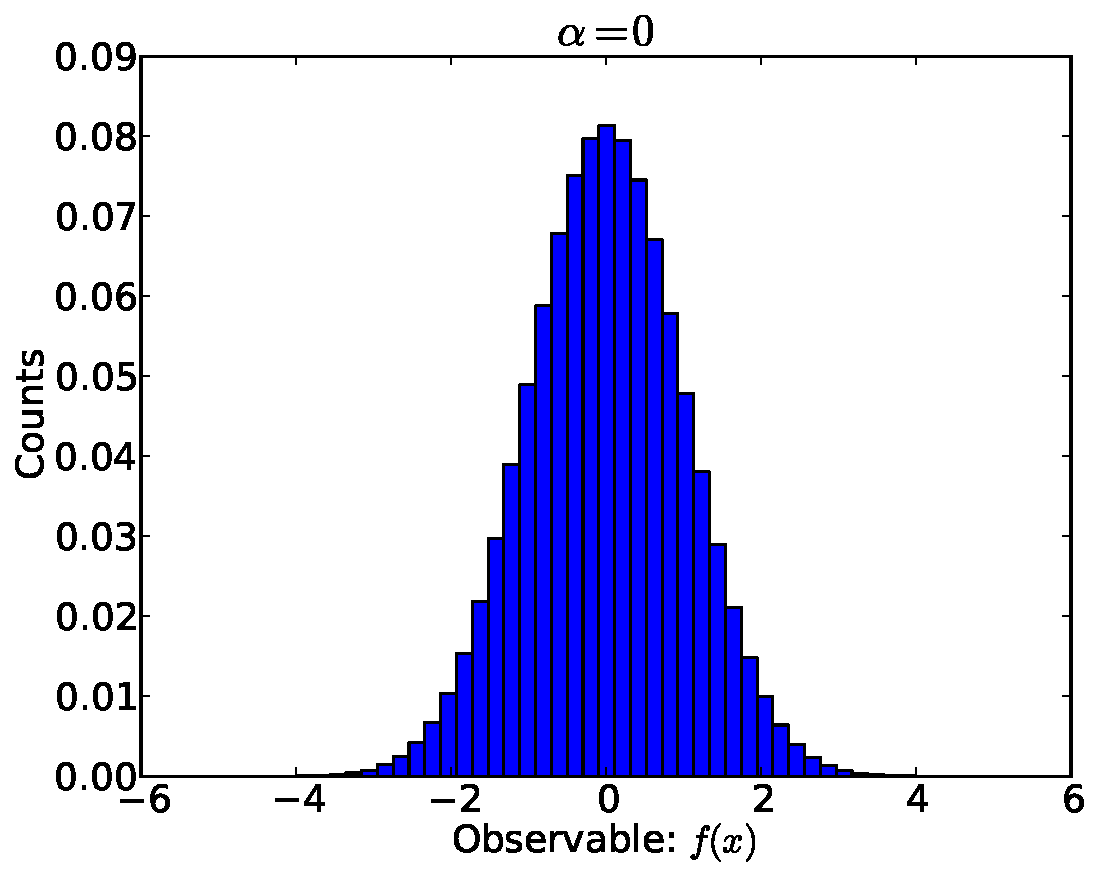
\includegraphics[width=5.0cm]{figures/model_hist0.pdf}
}
\subfigure[]{
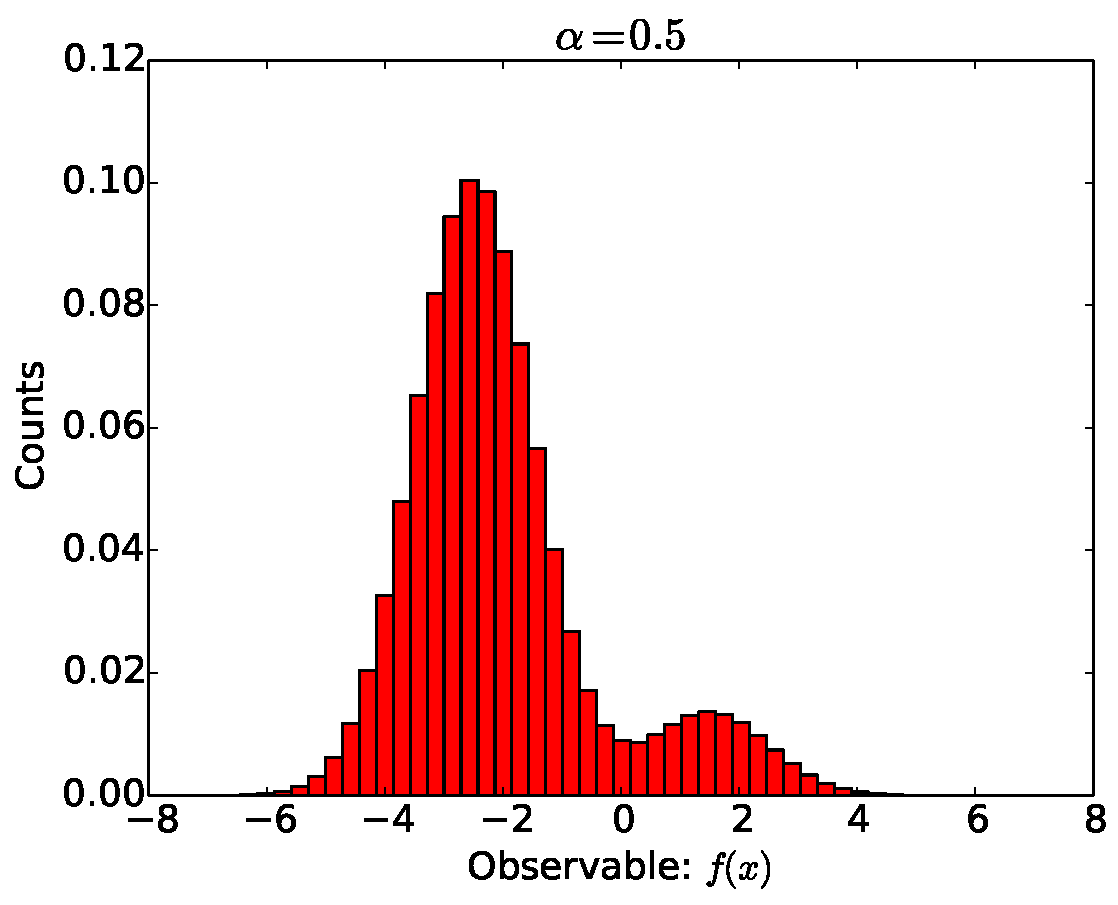
\includegraphics[width=5.0cm]{figures/model_hist2.pdf}
}
\caption{
Raw ($\alpha = 0$) and reweighted (e.g. tilted) histograms of a one dimensional observable.
}
\label{figure:Hist}
\end{figure}

With the equilibrium populations, we can calculate the equilibrium expectations of an arbitrary observable $h(x)$:

$$\langle h(x)\rangle _\alpha = \sum_j h(x_j) \pi_j(\alpha)$$

In the above bracket notation, $\langle h(x)\rangle _\alpha$ is the ensemble average of $h(x)$ in an ensemble that is perturbed by a biasing potential $\Delta U(x;\alpha)$.  At this point, the determination of $\alpha$ has not yet been discussed.  The key idea, however, is that the $\alpha$ reweighted ensemble $\langle \rangle _\alpha$ should recapitulate the experimental measurements:

$$\langle f_i(x)\rangle _\alpha \approx F_i$$


\subsection{A likelihood framework}

We now derive a likelihood framework for determining the coefficients $\alpha$ used in the biasing potential.  Given adequate sampling and self-consistent experiments, there should exist some \emph{true} value of $\alpha$ whose ensemble matches the experimental data.  However, experimental uncertainty ($\sigma_i)$ prevents exact agreement between the measurements and the true ensemble.  For the models in the current work, we model $\sigma_i$ as the uncertainty associated with predicting chemical shifts and scalar couplings from structures; this dominant error is quantified by the RMS uncertainty estimated during the parameterization of chemical shift and scalar coupling models.  We use an independent normal approximation (see Appx. S3) to model the agreement between the $\alpha$ ensemble and the measurements:

$$P(F_i | \alpha) \sim N(\langle f_i(x)\rangle _\alpha, \sigma_i^2)$$

Using Bayes Theorem, we can calculate the posterior distribution of $\alpha$:

$$P(\alpha | F_1, ..., F_n) \propto P(F_1, ..., F_n | \alpha) P(\alpha)$$

Now we let $LP(\alpha)$ denote the log posterior of $\alpha$ and simplify, dropping terms that are independent of $\alpha$:

$$LP(\alpha) = \log[ P(\alpha|F_1, ..., F_n)] = -\sum_i^n \frac{1}{2\sigma_i^2}(\langle f_i(x)\rangle _\alpha - F_i)^2 + \log P(\alpha)$$

Note the simple form of the log posterior.  The first term (i.e. the likelihood) measures the $\chi^2$ agreement between the reweighted ensemble and measurements.  The second term is the log of the prior distribution on $\alpha$.  In the present work, we evaluate two different choices of prior, finding similar results for each.  The first is the maximum entropy prior, which penalizes ensembles as they deviate from the raw simulation results:

$$\log P_{maxent}(\alpha) = \lambda \sum_j^m \pi_j(\alpha) \log \pi_j(\alpha)$$

The second prior we consider is a multivariate normal prior: $P_{MVN}(\alpha) \sim N(0, \Sigma)$.  The value of $\Sigma$ is given by $\Sigma_{ij} = \lambda Cov(f_i(x), f_j(x))$, as derived in Appx. S4.

Both priors can be used to achieve regularization, which is a powerful technique to reduce overfitting.  With large values of $\lambda$, both priors favor the raw simulation results (i.e. uniform conformational populations): $\pi_i \approx \frac{1}{n}$.  The value of $\lambda$ can be chosen via cross-validation or other methods (see Appx. S5).  

\subsection{Bayesian Modeling of Structural Ensembles}

Because ensemble inference often presents many plausible solutions \cite{fisher2010, rieping2005}, we avoid statistical methods that return a single solution (e.g. maximum likelihood).  We therefore use Markov chain Monte Carlo (MCMC), as implemented in PyMC \cite{patil2010pymc}, to sample the distribution of structural ensembles consistent with experiment.  The result is an ensemble of ensembles--a statistical ensemble of conformational ensembles.  Averaging all MCMC samples provides posterior mean  estimates of arbitrary structural features.  Similarly, examining the MCMC variances provides statistical uncertainties of equilibrium or structural features.  A Bayesian bootstrapping procedure \cite{rubin1981} can also be used to model the statistical uncertainty of the MD simulations (see Appx. S6).

\section{Results}

\subsection{Conformational Propensities of Trialanine}

Short peptides provide crucial tests for evaluating and optimizing molecular dynamics force fields \cite{Graf2007,beauchamp2012protein, Nerenberg2011, Best2008, Grdadolnik2011}.  Such peptides offer a window into the intrinsic conformational propensities of amino acids, free from the secondary structure bias found in statistical surveys of protein structures \cite{Jha2005}.  Here, we use BELT to infer the conformational populations of trialanine from chemical shift and scalar coupling measurements \cite{Graf2007}.  

Trialanine was simulated (see Methods) in five different force fields; six experimental measurements (three scalar couplings, three chemical shifts) probing the central alanine residue were used to construct a BELT ensemble.  The five force fields show considerable variation in their agreement with experiment (Fig. \ref{figure:ChiSquared}).  The amber96, amber99, charmm27, and oplsaa force fields, for example, initially show significant deviation from the experimental measurements.  Upon reweighting, however, all five force fields agree with experiment--including experiments that were \emph{not} used to fit the model (Fig. \ref{figure:ChiSquared}b).  Additionally, these results are robust to differences in the prior placed on $\alpha$.

\begin{figure}
\subfigure[]{
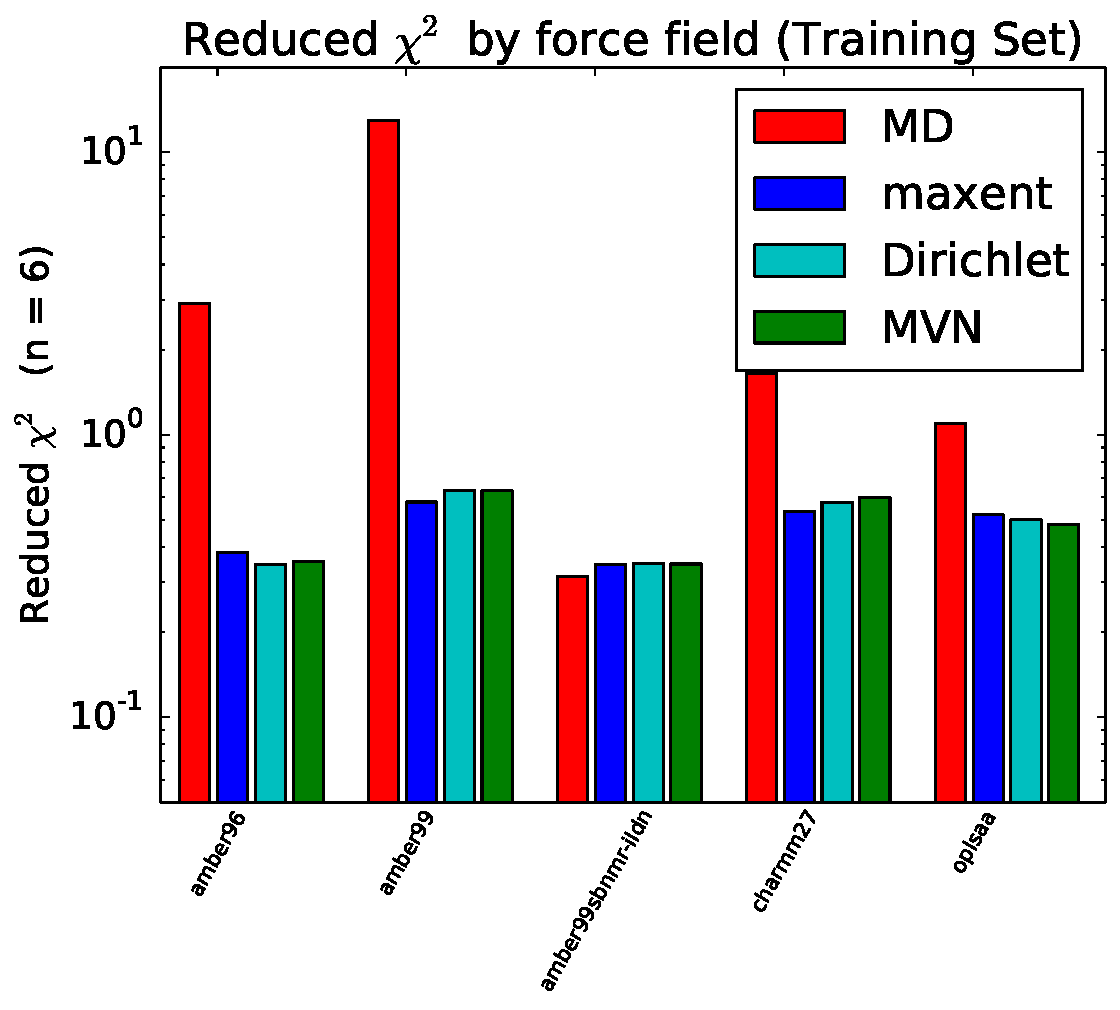
\includegraphics[width=7.5cm]{figures/chi2_train_priors.pdf}
}
\subfigure[]{
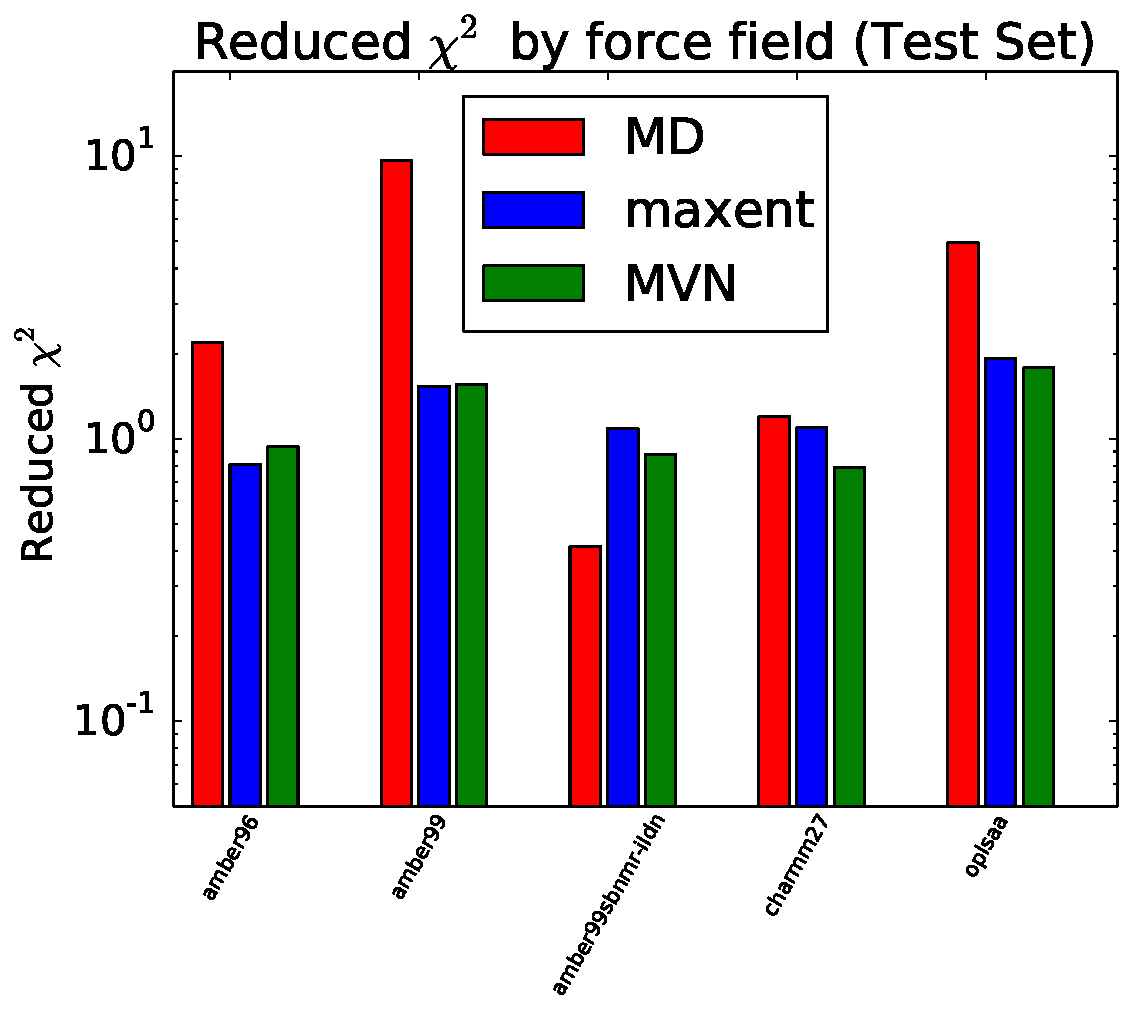
\includegraphics[width=7.5cm]{figures/chi2_test_priors.pdf}
}
\caption{
The reduced $\chi^2$ error (e.g. $\frac{\chi^2}{n}$) for MD and BELT (maxent and MVN priors) models.  The BELT reduced $\chi^2$ is estimated as the mean reduced $\chi^2$ over all MCMC samples.  (a).  Calculated using the six measurements used to fit the BELT model.  (b).  Calculated using four measurements \emph{not} used to fit the BELT model.  See Methods for the definition of training and test sets.
}
\label{figure:ChiSquared}
\end{figure}



\begin{figure}
\subfigure[]{
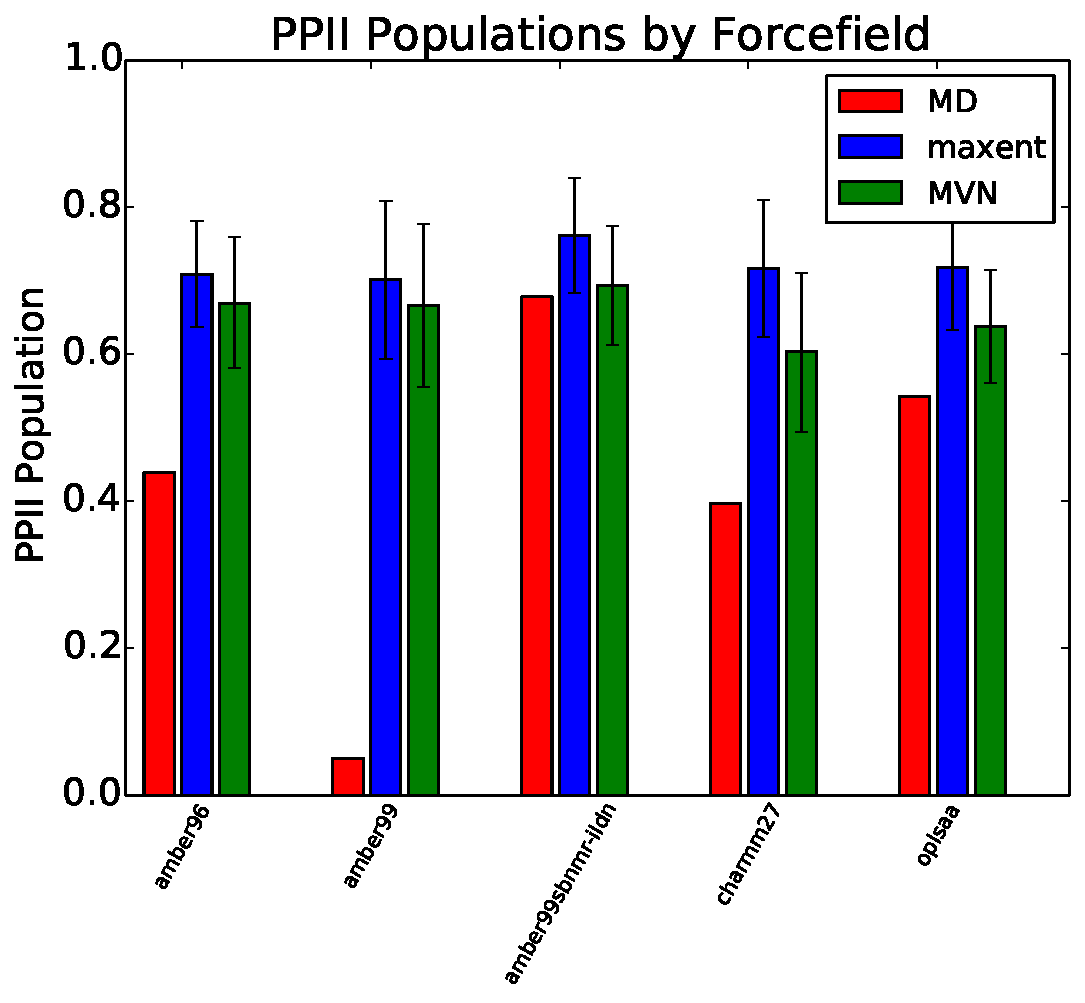
\includegraphics[width=7.5cm]{figures/state_0_by_forcefield_priors.pdf}
}

\subfigure[]{
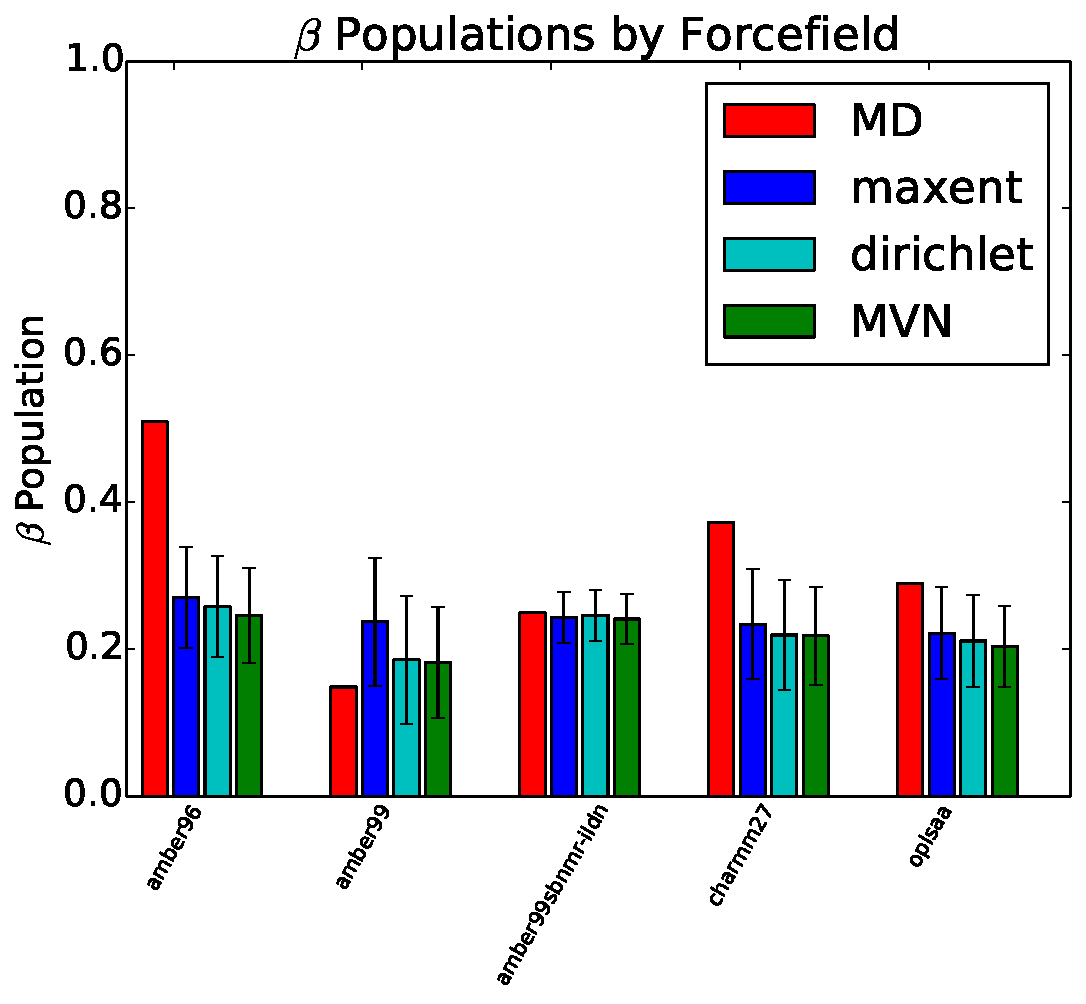
\includegraphics[width=7.5cm]{figures/state_1_by_forcefield_priors.pdf}
}
\subfigure[]{
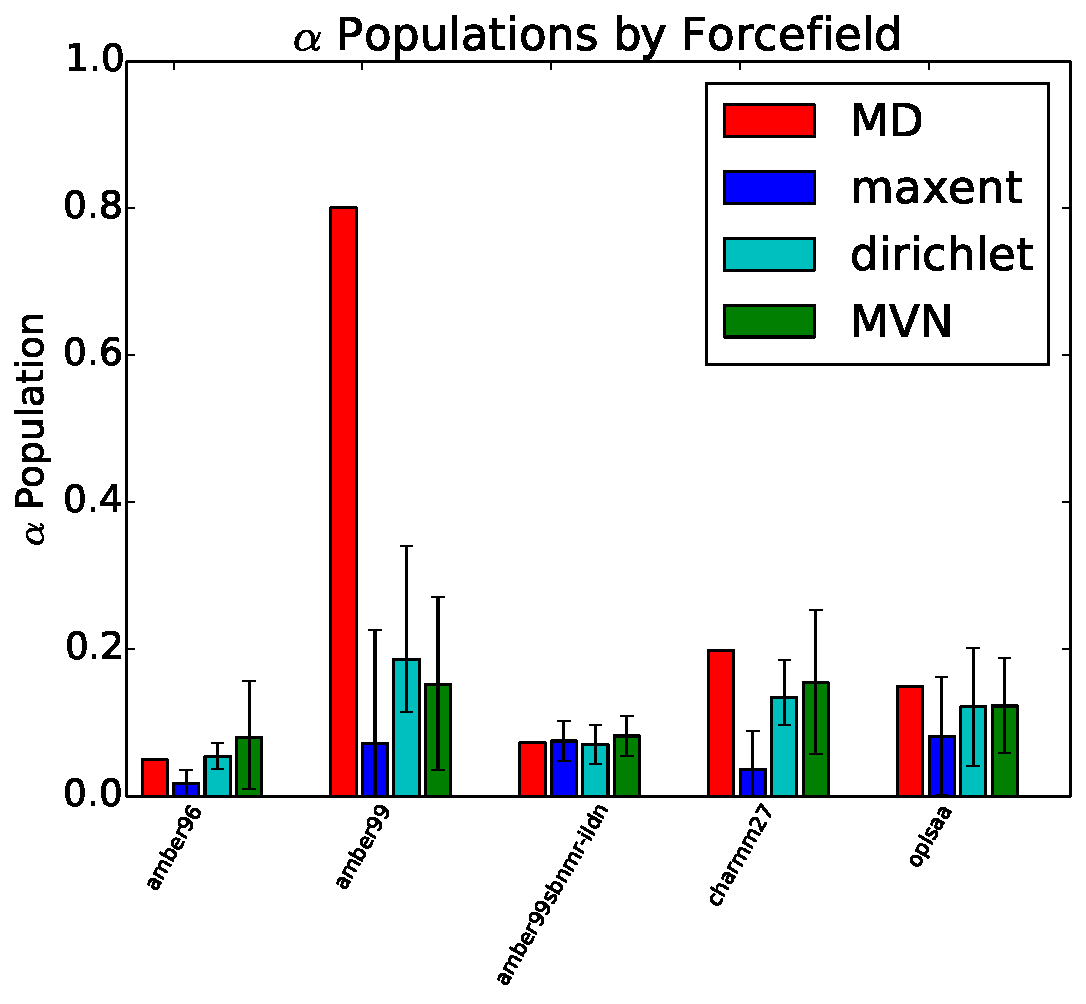
\includegraphics[width=7.5cm]{figures/state_2_by_forcefield_priors.pdf}
}
\caption{
MD and BELT (maxent and MVN priors) conformational propensities for each force field.  
}
\label{figure:ALA3}
\end{figure}


\begin{figure}
\subfigure[]{
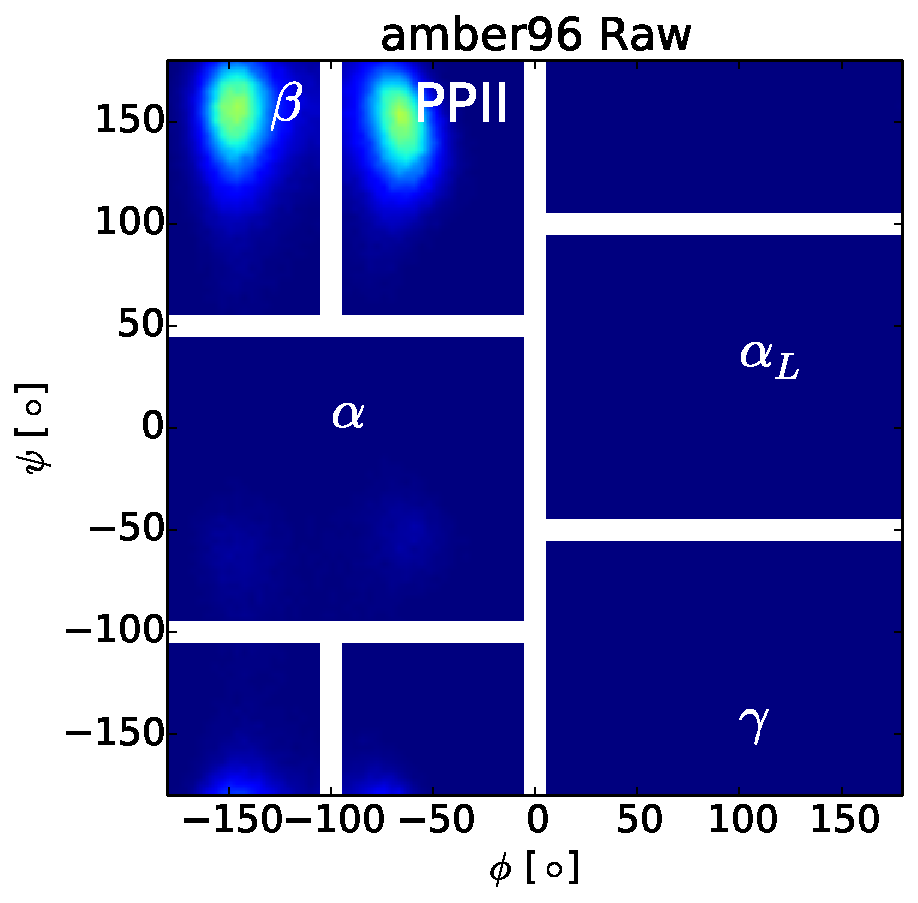
\includegraphics[width=5.05cm]{figures/ALA3_rama_amber96_raw.pdf}
}
\subfigure[]{
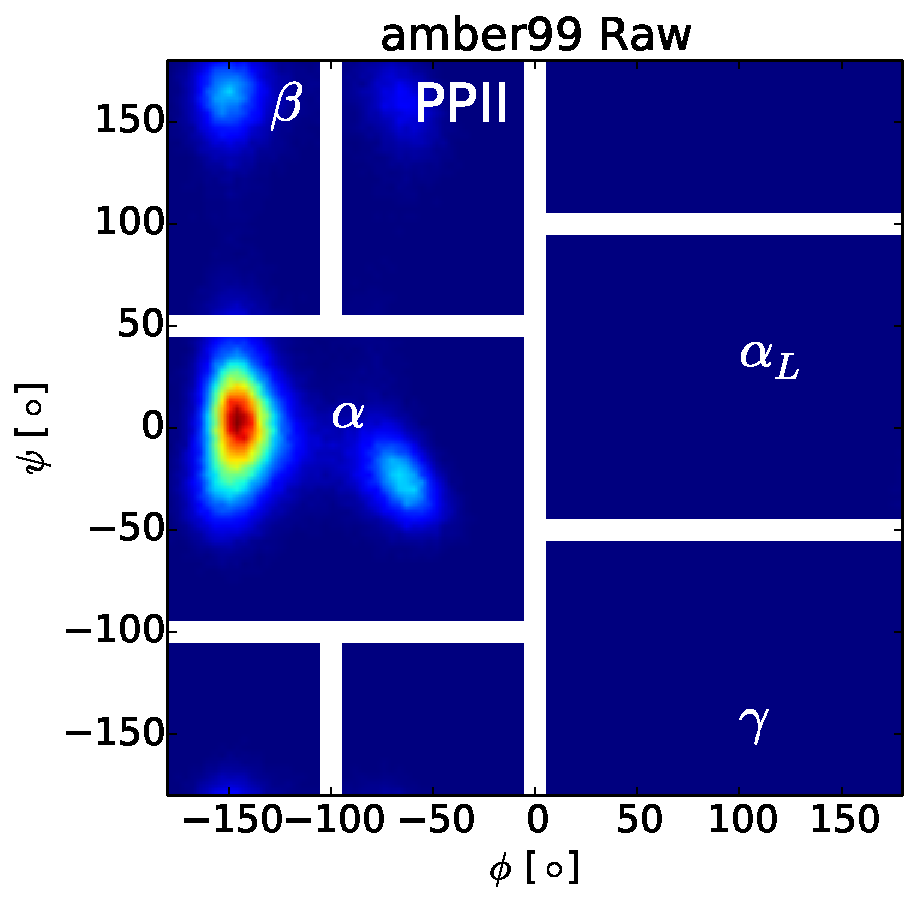
\includegraphics[width=5.05cm]{figures/ALA3_rama_amber99_raw.pdf}
}
\subfigure[]{
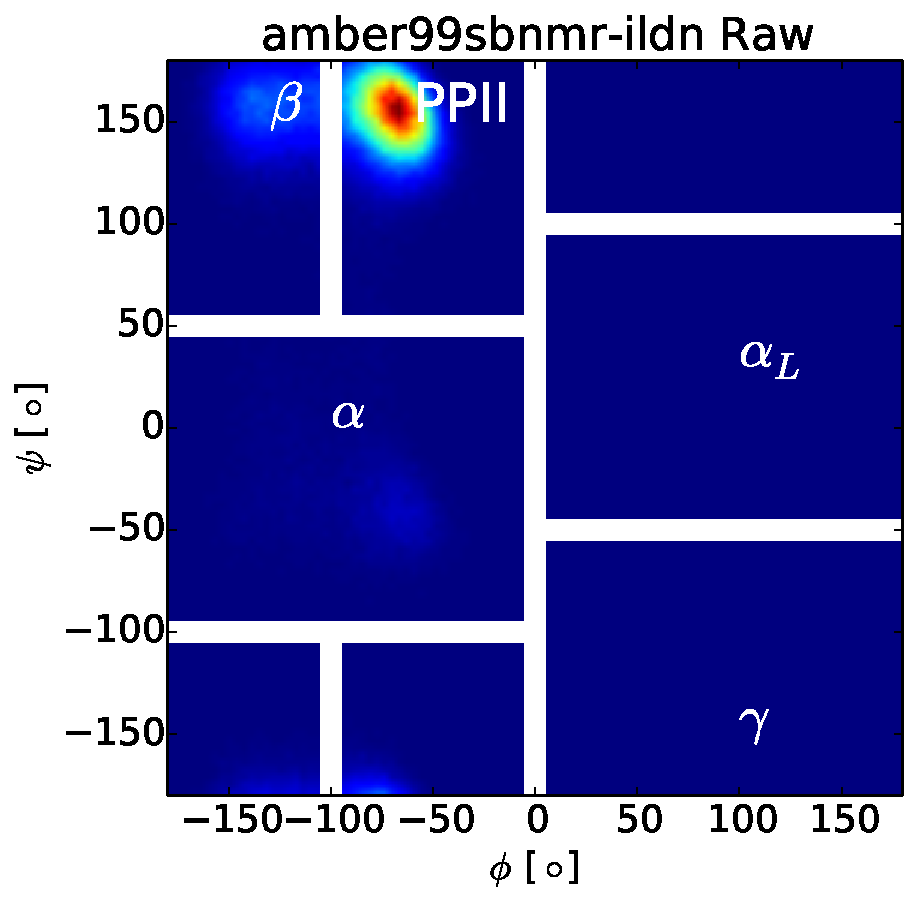
\includegraphics[width=5.05cm]{figures/ALA3_rama_amber99sbnmr-ildn_raw.pdf}
}

\subfigure[]{
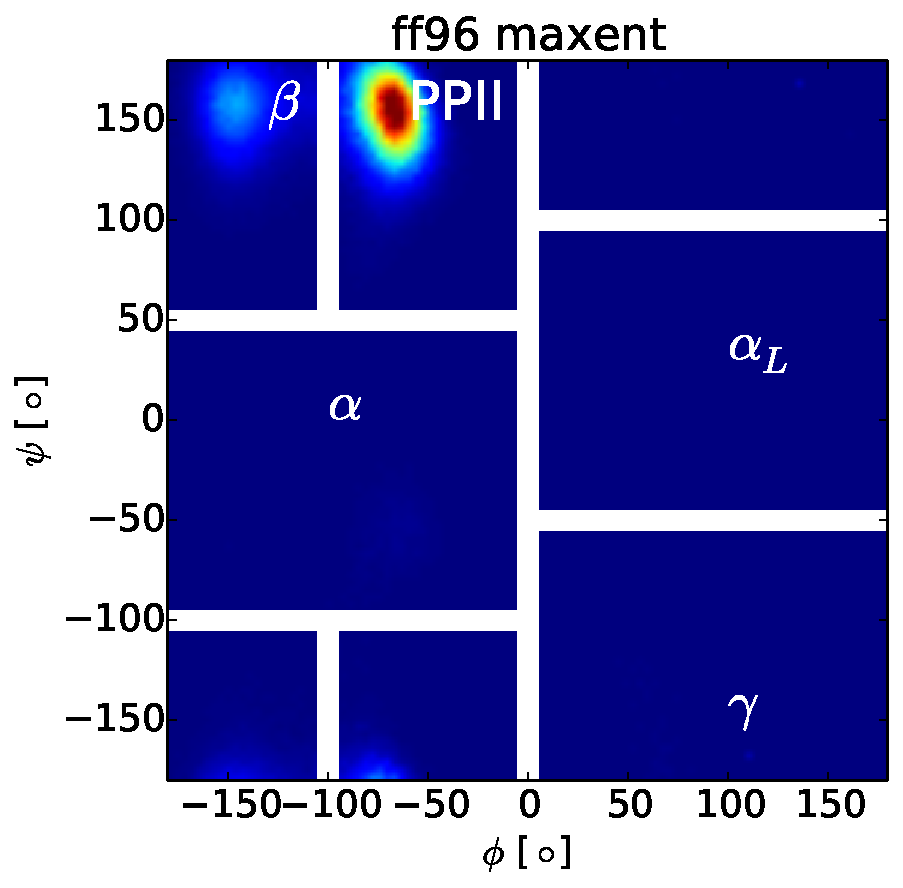
\includegraphics[width=5.05cm]{figures/ALA3_rama_amber96_maxent_belt.pdf}
}
\subfigure[]{
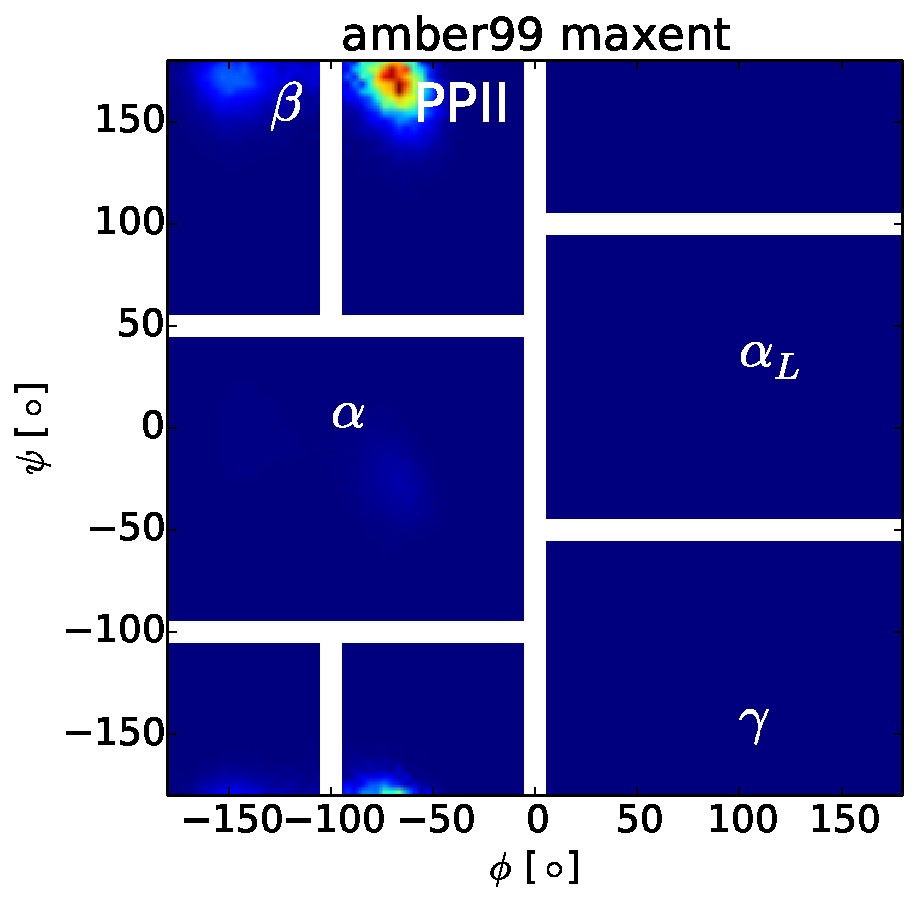
\includegraphics[width=5.05cm]{figures/ALA3_rama_amber99_maxent_belt.pdf}
}
\subfigure[]{
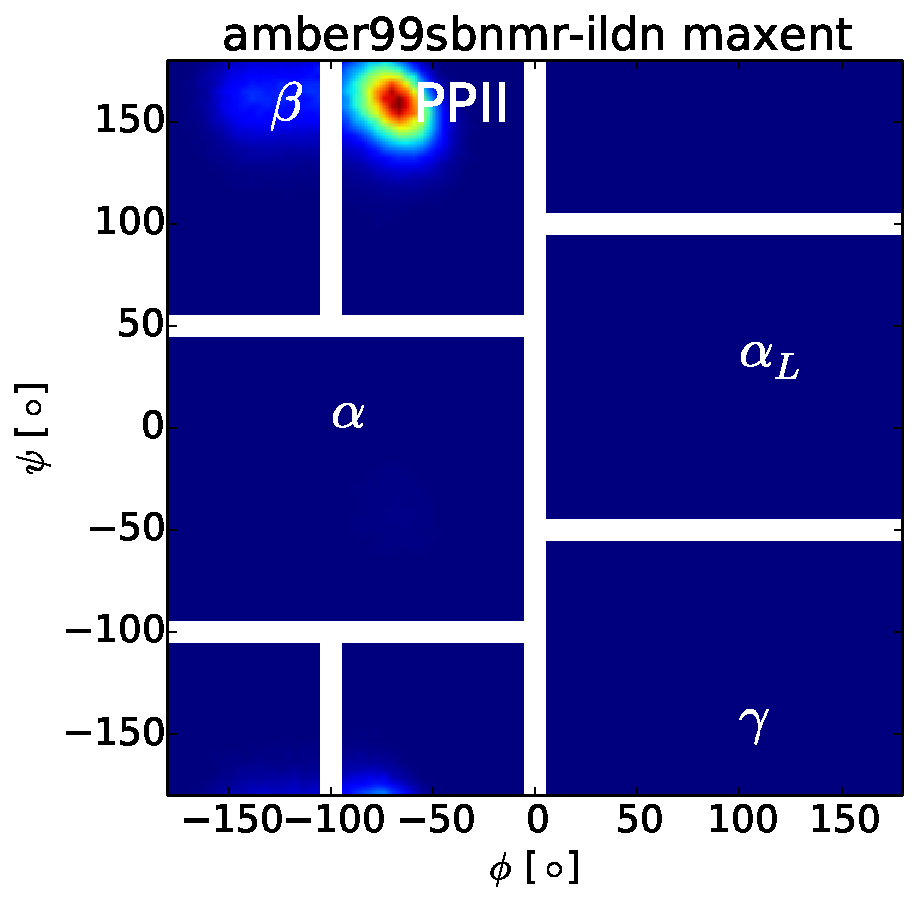
\includegraphics[width=5.05cm]{figures/ALA3_rama_amber99sbnmr-ildn_maxent_belt.pdf}
}

\subfigure[]{
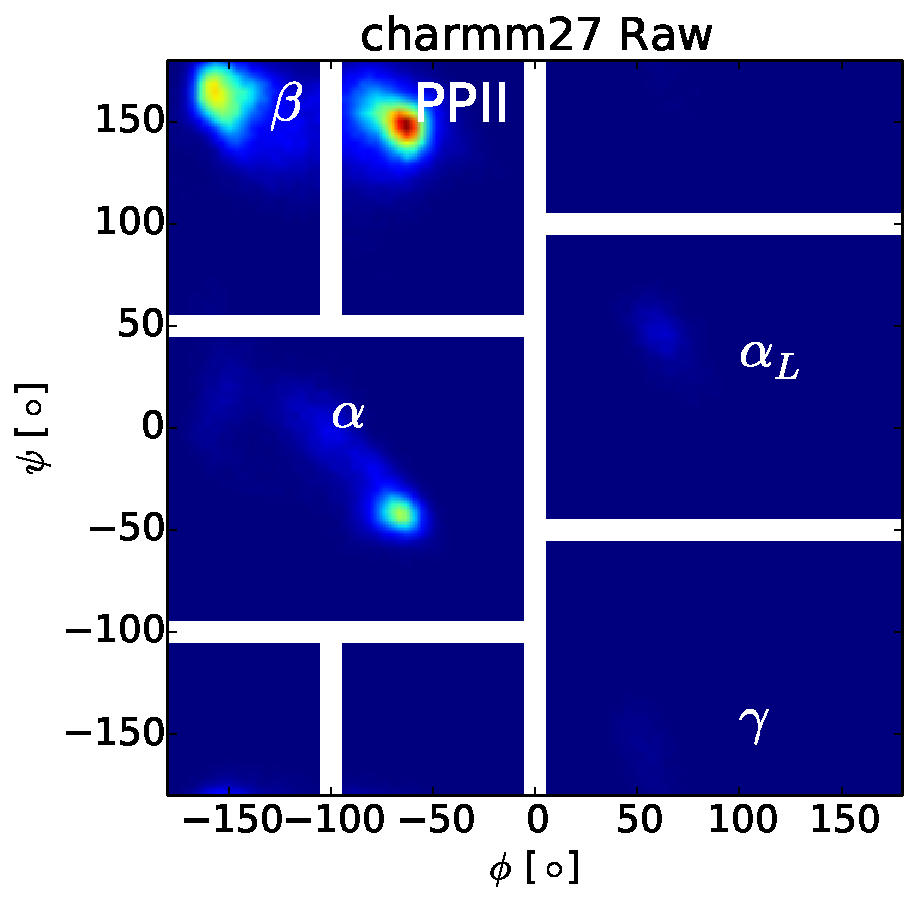
\includegraphics[width=5.05cm]{figures/ALA3_rama_charmm27_raw.pdf}
}
\subfigure[]{
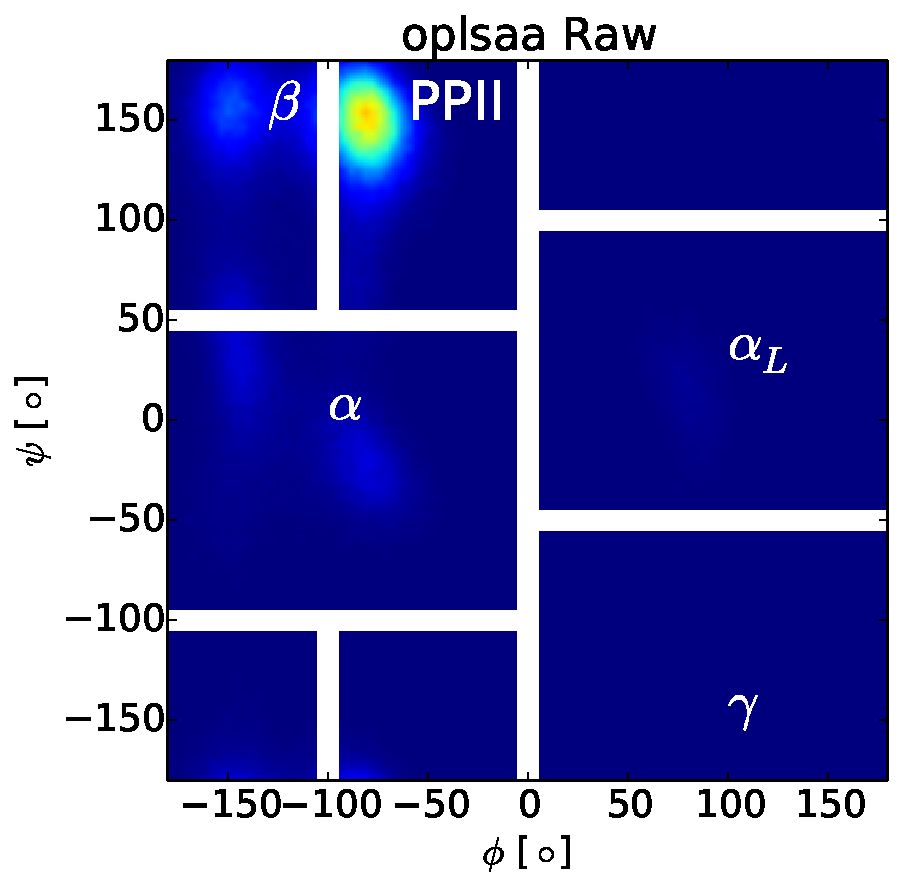
\includegraphics[width=5.05cm]{figures/ALA3_rama_oplsaa_raw.pdf}
}

\subfigure[]{
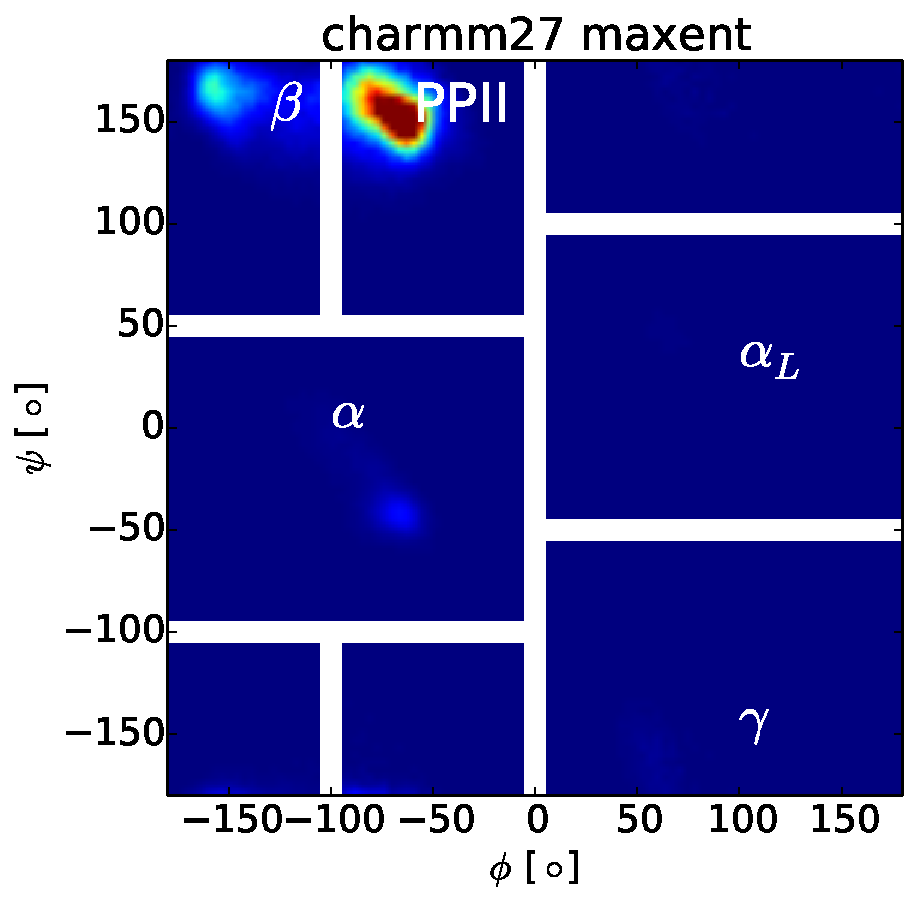
\includegraphics[width=5.05cm]{figures/ALA3_rama_charmm27_maxent_belt.pdf}
}
\subfigure[]{
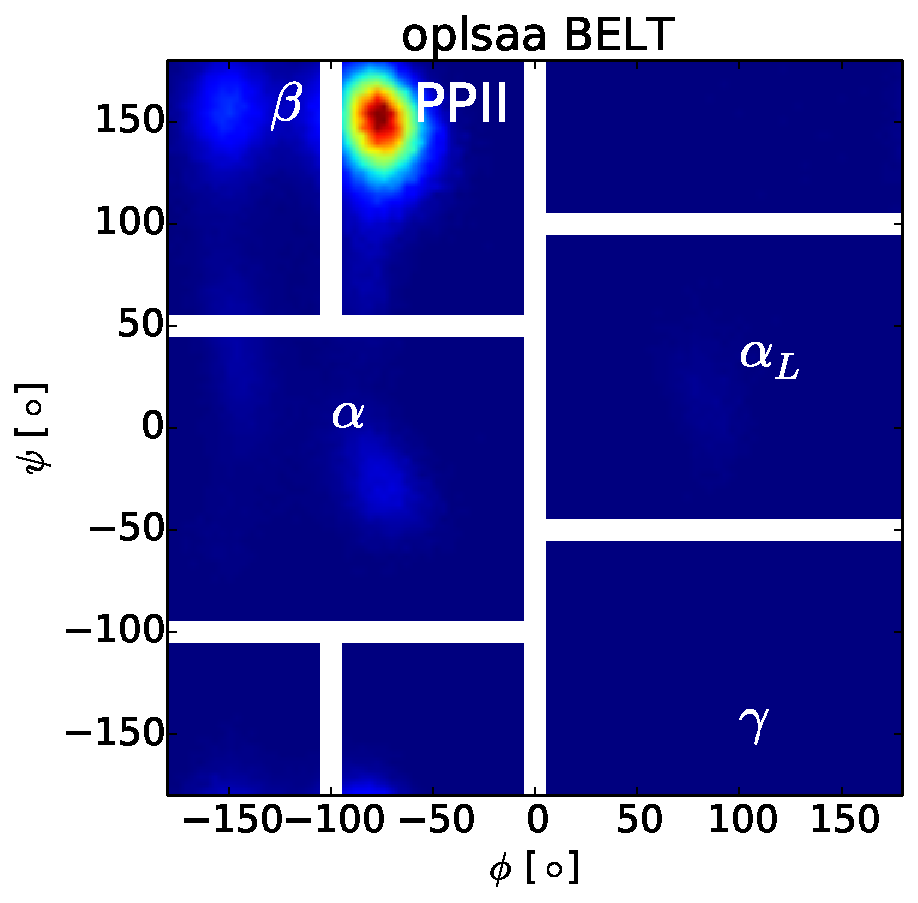
\includegraphics[width=5.05cm]{figures/ALA3_rama_oplsaa_maxent_belt.pdf}
}

\caption{
Ramachandran plot of MD and BELT (maxent prior) ensembles for each force field.  Comparison of BELT models with different priors (maxent and MVN) are given in Fig. S1.  
}
\label{figure:Rama}
\end{figure}

Several independent experimental studies have shown that short alanine peptides prefer the polyproline type helix (PPII) in solution \cite{Grdadolnik2011, Graf2007, Avbelj2006}.  Most molecular dynamics force fields, however, are known to underpopulate the PPII state \cite{Graf2007,beauchamp2012protein,Nerenberg2011, Best2008}.  Our trialanine simulations recapitulate this known deficiency (Fig. \ref{figure:ALA3}; red), with amber96 showing a strong $\beta$ bias (Fig. \ref{figure:ALA3}b) and amber99 showing a strong $\alpha$ bias (Fig. \ref{figure:ALA3}c).  However, combining simulation and experiment leads to conformational ensembles that are robust to differences in force field and prior (Fig. \ref{figure:ALA3}; green and blue).  Full Ramachandran plots of the $(\phi, \psi)$ preferences (Fig. \ref{figure:Rama}) reveal similar features in all five BELT models.  

\subsection{Bayesian Inference allows Ambiguous Experiments}

BELT allows the full characterization of posterior distributions using MCMC.  Most previous approaches, however, have focused on obtaining point estimates of conformational ensembles \cite{rozycki2011saxs,  Graf2007}.  In many cases, however, ambiguous experimental data precludes a point-estimate of the conformational ensemble.  To illustrate this point, we plot the measured \cite{Graf2007} value of $^3J(H_NH_\alpha)$ in the context of the Karplus equation relating $\phi$ to $^3J(H_NH_\alpha)$.  The measured coupling corresponds to four \emph{different} values of $\phi$ (Fig. \ref{figure:Ambiguity}a), suggesting that a point estimate is inappropriate for modeling conformations or ensembles.  As a concrete example of bimodality, we calculated the posterior distribution of $PP_{II}$ for the amber99 force field reweighted with two ($^3J(H_NH_\alpha)$, $^3J(H_NC')$) NMR measurements (Fig. \ref{figure:Ambiguity}b).  The observed bimodal distribution indicates the need to fully characterize the posterior 
distribution.  

\begin{figure}
\subfigure[]{
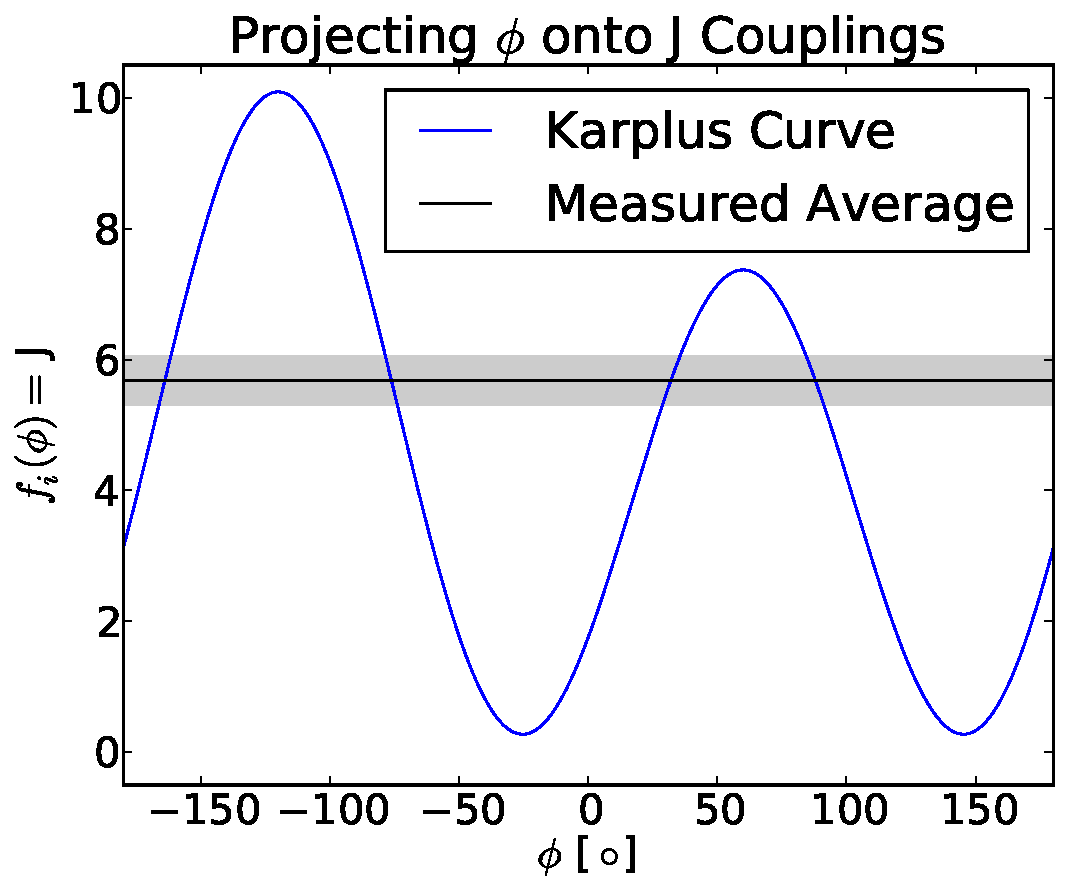
\includegraphics[width=7.5cm]{figures/single_karplus.pdf}
}
\subfigure[]{
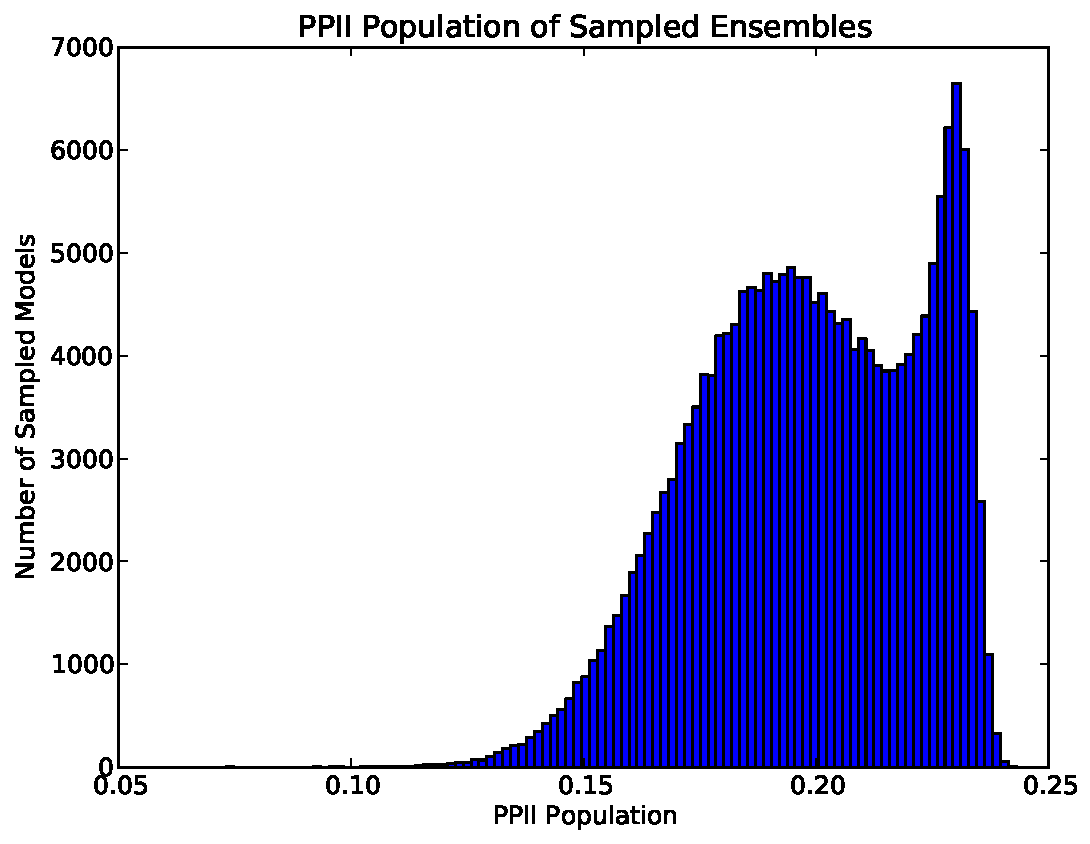
\includegraphics[width=7.5cm]{figures/amber99_PPII_histogram.pdf}
}
\caption{
(a).  The Karplus equation connecting the backbone torsion $\phi$ to $^3J(H_NH_\alpha)$ is ambiguous; observed values of $^3J(H_NH_\alpha)$ are consistent multiple conformations.  (b).  BELT modeling (amber99 force field) with two measurements ($^3J(H_NH_\alpha)$, $^3J(H_NC')$) shows a bimodal posterior.  
}
\label{figure:Ambiguity}

\end{figure}



\section{Discussion}

\subsection{Structural (Ensemble?) Biology}

Why model structural ensembles, rather than just structures?  At least three compelling reasons favor ensembles.  First, biological molecules are multi-state machines that fold, unfold, bind ligands, aggregate, and change conformation.  Biology is controlled by the relative populations of these states.  Ensembles capture aspects of these phenomena by encoding equilibrium populations with structures.  A second argument for ensemble modeling is fidelity to experiment.  Most solution experiments measure ensemble average equilibrium properties--chemical shifts, scalar couplings, NOEs, SAXS, and FRET are reasonably well-described as equilibrium properties.  A truly quantitative connection to these measurements requires modeling the equilibrium ensemble.  Finally, recent advances in atomistic simulation \cite{hess2008, pronk2013gromacs, eastman2012openmm, eastman2010openmm}, special-purpose hardware \cite{Shaw2008}, and distributed computing analysis \cite{emma, msmb2} have enabled atomistic simulations to reach 
the millisecond timescale \cite{voelz2010, bowman2011atomistic, shaw2010, Shaw2011}; the computational cost of ensemble modeling is quickly becoming manageable.

One might argue that structural ensembles are unnecessary because many proteins occupy a single state under physiological conditions.  For such proteins, it is probably safe to enforce single state behavior, as is done in current modeling approaches. However, we suggest that the number of states be \emph{inferred}--not \emph{assumed}.  


\subsection{Resolving Fine Structure may Require Improved Observables}

The five BELT ensembles show quantitative agreement in $\alpha$, $\beta$, and $PP_{II}$ populations (Fig. \ref{figure:ALA3}).  However, the finer details of each Ramachandran plot (Fig. \ref{figure:Rama}) suggest subtle differences between the 
five models.  Because all five BELT ensembles show excellent agreement with experiment (Fig. \ref{figure:ChiSquared}), we conclude that current predictors of chemical shifts and scalar couplings are insufficiently precise to resolve (and falsify) subtle force field differences.  The most obvious such difference is the width, shape, and orientation of the $PP_{II}$ basin.  Most strikingly, amber96 and oplsaa have $PP_{II}$ basins that are vertically oriented, while amber99, amber99sbnmr-ildn, and charmm27 show diagonally oriented $PP_{II}$ basins.  This highlights the need for more sensitive connections between simulation and experiment, such as chemical shift and scalar coupling models.


\subsection{Comparison to Previous Ensemble Methods}

BELT offers several key advantages over previous ensemble estimation techniques.  Most previous ensemble modeling efforts involve a protocol with three key ingredients: clustering, a $\chi^2$ objective function, and population inference on the clusters.  For example, this recipe describes the approach used in previous analyses of homopeptides \cite{Graf2007}, the EROS technique for SAXS modeling \cite{rozycki2011saxs}, and the Bayesian Weighting formalism \cite{fisher2010}.  In our opinion, the primary disadvantage of these techniques is the need for a clustering step.  Clustering can introduce two different errors, depending on whether the number of clusters is small or large.  In the limit of few states, clustering can overly coarsen the system of interest, possible preventing the model from reproducing multiple experimental observables.  At the other extreme, too many states could lead to over-fitting when estimating the many populations required to parameterize the model.  This will lead to poor generalization performance and large errors when predicting experiments \emph{not} used to train the model.  

In contrast, BELT avoids clustering by projecting simulations onto a basis defined by the predicted experimental observables.  The advantage of working in this basis are fourfold. First, in BELT, one estimates a single parameter ($\alpha_i$) for each experimental observable.  If the number of experiments is small, as is often the case, the inference problem involves only a few parameters.  Second, the predicted observables are a \emph{natural} basis for biophysical calculations.  This basis allows direct connection to experiment and often provides insight into the molecular interactions driving biophysical phenenoma.  For example, the projection onto observables could be used to rationally infer force field parameters, similar to the ForceBalance method \cite{wang2012, wang2013systematic}.  Third, suppose two conformations have the same predicted experimental observables.  In BELT, these conformations will have the same population.  In clustering based methods, the populations of these conformations could vary simply due to random fluctuations.  Finally, in the limit of exact measurements, BELT reduces to a previous \cite{chodera2012} maximum entropy approach (see Appx. S1).  

We also point out some surprising differences between BELT and BW-like methods.  BW-like methods have the interesting property that the in-state means of features are preserved.  More precisely, suppose that $\chi_s(x)$ is the indicator function of a conformational state $s$.  Then in-state averages of the form $<h(x) \chi_s(x)>$ do \emph{not} depend on the reweighted populations.  BELT, however, does not preserve the in-state averages; in fact, this property is the direct result of BELT's connection to maximum entropy modeling (see Appx. S1 and ref. \cite{chodera2012}).  The effect of this property is that the ``peaks'' of reweighted histograms are slightly shifted relative to the raw MD results, as observed in Fig. \ref{figure:Hist}.  

\subsection{Quantitative Comparison of Ensemble Inference Techniques}

The above reasons provide theoretical arguments supporting the BELT method.  However, it is possible to evaluate the method \emph{quantitatively}.  One hallmark of a good statistical model is its predictive ability on set-aside test data \cite{friedman2001elements}.  We therefore evaluated BW (see Methods) and BELT models on set-aside test data.  

For all five force fields, BELT produces models that give statistical agreement with experiment on the test data.  For three out of five force fields, BELT gives the \emph{best} model.  The BELT prior appears relatively unimportant.  In cases where BELT outperforms BW, it does so significantly.  

For the two remaining cases, BW outperforms BELT.  For these force fields (amber99sbnmr-ildn and charmm27), however, all four models (BW, BELT-MVN, BELT-maxent), and MD) are consistent ($\chi^2 \lesssim 1$) with experiment.  We conclude that while both BW and BELT provide provide reasonable models, BELT gives better models in situations with poor starting force fields.  

\begin{tabular}{lrrrrr}
\toprule
   &               amber96 &  amber99 &  amber99sbnmr-ildn &  charmm27 &  oplsaa \\
\midrule
Method (Prior)&          &          &                    &           &         \\
BW            &     0.67 &     1.73 &           \bf{0.46}&  \bf{0.47}&    2.75 \\
BELT  (MVN)   &     0.62 &     0.90 &               0.66 &      0.76 &\bf{0.91} \\
BELT  (maxent)&\bf{0.50} &\bf{0.80} &               0.61 &      0.76 &    1.11 \\
MD            &     2.18 &     9.63 &               0.41 &      1.20 &    4.93 \\
\bottomrule
\end{tabular}


\section{Future Work}

The BELT method can be extended in several ways.  We have already worked out some of these extensions.  In App. S3, we derive an approximate correction for working with dependent data.  Another obvious extension is the use of non-Normal error models.  These models can be directly inserted into the current framework by replacing the $\chi^2$ term in the likelihood with some other loss function.  More sophisticated models could separately treat the uncertainties associated with predicting observables and the uncertainties of conformations.  This would replace the regularization and Bayesian Bootstrapping (App. S6) approaches used herein.  Another promising avenue is to combine Bayesian modeling of structural ensembles with Bayesian models for experimental observables.  A Bayesian formalism for NMR experients has previously been developed \cite{rieping2005, habeck2006}; connecting BELT to these methods may be straightforward.  


\section{Conclusion}

Bayesian Energy Landscape Tilting allows the simultaneous characterization of structural and equilibrium properties.  Through its use of MCMC, BELT is robust to ambiguous experiments and provides rigorous uncertainty estimates.  BELT models constructed with a handful of NMR measurements correct significant force field bias and provide generalizable, \emph{force field independent} trialanine ensembles.  


\section{Acknowledgements}

We thank John Chodera, TJ Lane, Frank Cochran, Pehr Harbury, Xuesong Shi, and Dan Herschlag for helpful discussions.  

\section{Methods}

\subsection{Molecular Dynamics Simulations}

Trialanine was simulated in the amber96\cite{kollman1996}, amber99\cite{wang2000}, amber99sbnmr-ildn\cite{li2010}, charmm27\cite{mackerell2004extending,bjelkmar2010implementation}, and oplsaa\cite{kaminski2001evaluation} force fields, as previously reported \cite{beauchamp2012protein}.  Simulations were performed using Gromacs 4.5 \cite{hess2008} and run at constant temperature (300 K) and pressure (1.01 atm).  Each simulation was at least 225 ns long.  Conformations were stored every 1 ps.  

\subsection{Chemical Shift and Scalar Couplings}

All NMR measurements in this work refer to experiments \cite{Graf2007} probing the central residue of trialanine.  We chose to focus on this residue because it will be most robust to pH dependent effects, which may be difficult to model with current force fields.  

Chemical shifts (H, HA, CA, CB) for each frame were calculated using the average prediction of ShiftX2\cite{han2011shiftx2}, SPARTA+ \cite{Shen2010}, and PPM\cite{li2012ppm}; uncertainties for each model were estimated using their reported RMS prediction errors.  Overall uncertainties were estimated as $\sqrt{\sum w_i \sigma_i^2}$, where $w_i \propto \frac{1}{\sigma_i^2}$ is the weight (e.g $\sum_i w_i = 1$) of each chemical shift model and $\sigma_i$ is the uncertainty of each chemical shift model.  The J couplings were calculated using the following Karplus relations: $^3J(H^N C')$ \cite{Schmidt1999}, $^3J(H^N H^\alpha)$ \cite{vogeli2007limits}, $^2J(N C^\alpha)$ \cite{Graf2007}, $^3J(H^\alpha C')$ \cite{Schmidt1999}, $^1J(N C^\alpha)$ \cite{Graf2007}, $^3J(H^N C^\beta)$ \cite{vogeli2007limits}.  J coupling uncertainties were approximated as the RMS errors reported when fitting the Karplus coefficients.  

We have divided the available experimental measurements into a training and test set, with the training set consisting of $^3J(H^N C')$,  $^2J(N C^\alpha)$, $^3J(H^N C^\beta)$ scalar couplings and the $C_\alpha$, the $H$, and the $C_\beta$ chemical shifts.  The test set consists of $^3J(H^N H^\alpha)$, $^3J(H^\alpha C')$, and $^1J(N C^\alpha)$.  The division into training and test sets serves three purposes.  First, it provides a test of overfitting.  Second, it allows us to reduce the computational cost of BELT calculations.  Third, it allows us to train on data that is approximately uncorrelated; BELT is best suited for working with uncorrelated data.  Additional suggestions for data curation are provided in Appx. S7.  

\subsection{BELT}

All BELT calculations were performed using the FitEnsemble package (\url{https://github.com/kyleabeauchamp/FitEnsemble}).  The online FitEnsemble tutorial demonstrates the use of BELT with a single experimental measurement ($^3J(H^N H^\alpha)$).  Source code for calculations in this work will be made available at \url{https://github.com/kyleabeauchamp/EnsemblePaper}.  

Regularization strength was determined via cross validation as described in Appx. S5.  MCMC sampling for each of the current models the current work took approximately 12 hours.  These datasets used included six measurements and approximately 250,000 conformations.  For each model, we used PyMC to sample 5,000,000 values of $\alpha$; sampled values of $\alpha$ were thinned 100-fold to reduce correlation.  The first 5,000 samples (before thinning) are discarded as burn-in.  MCMC traces are shown in Fig. S2 and discussed in Appx. S8.  

\subsection{Bayesian Weighting}

Bayesian weighting models were constructed with four conformational states consisting of $\alpha$, $\beta$, $PP_{II}$, and other.  State definitions were taken from \cite{jha}.  1,000,000 MCMC samples were generated.  The first 5,000 were discarded as burn-in and the remainder were thinned 100-fold.  A dirichlet prior (with 1 count per state) was used to model the prior populations of each conformational state.  We point out that there are several varieties of BW-like models; our implementation is one of several possible choices of prior.  BW calculations were performed using the bayesian weighting module within FitEnsemble.  


\bibliography{belt}


\end{document}